\section{Algorithmic type rules}\label{section:typeruless}
%We are now ready to introduce type rules for a type checker of the type system in Baillot and Ghyselen \cite{BaillotGhyselen2021}. %TODO 
%
%
%A piecewise complexity $\kappa$ is a set of pairs $(\Phi_i, K_i)$ where $K_i$ is an index describing a complexity that is valid within the feasible region described by the set of constraints $\Phi_i$. As such, a piecewise complexity $\kappa = \{(\Phi_1, K_1), \cdots, (\Phi_n, K_n)\}$ describes a complexity bound within the feasible region $\mathcal{M}_\varphi(\Phi_1) \cup \cdots \cup \mathcal{M}_\varphi(\Phi_n)$ for some $\varphi$ such that $\Phi_1, \cdots, \Phi_n$ use index variables in $\varphi$. In the case where $m$ feasible regions $\mathcal{M}_\varphi(\Phi_{i_1})$, $\mathcal{M}_\varphi(\Phi_{i_{m-1}})$ and $\mathcal{M}_\varphi(\Phi_{i_m})$ intersect, we choose the maximal complexity of the corresponding complexities for any valuation $\rho$ in the intersecting region.\\

When typing a process, we often need to find an index that is an upper bound on two other indices, for which there may be many options. To allow for the type checker to be as precise as possible, we want to find the minimum complexity that is a bound of two other complexities, which will depend on the representation of complexity, and as such, instead of representing complexity bounds using indices, we opt to use sets of indices which we refer to as \textit{combined complexities}. Intuitively, given any point in the space spanned by some index variables, the combined complexity at that point is the maximum of the complexities making up the combined complexity at that point. This is illustrated in Figure \ref{fig:combined_complexity} which shows a combined complexity consisting of three indices. The red dashed line represents the bound on the combined complexity. Representing complexities as sets of indices has the effect of \textit{externalizing} the process of finding bounds of complexities by deferring this until a later time. We will later define the algorithm \textit{basis} that removes superfluous indices of a combined complexity. In Figure \ref{fig:combined_complexity} the index $K$ is superfluous as it never contributes to the bound of the combined complexity.

\begin{figure}
    \centering
    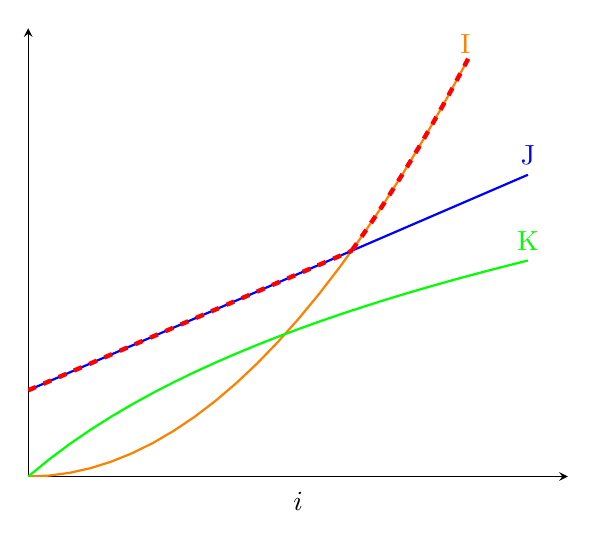
\begin{tikzpicture}
\begin{axis}[
    axis lines = left,
    xlabel = \(i\),
    ylabel = {},
    domain = 0:2.5,
    xtick={\empty},ytick={\empty},
    ymin=0,
    ymax=5.2,
    xmax=2.7,
    restrict y to domain=0:5,
]
    \addplot[thick, color=orange]{x^2} node[above,pos=1] {I};
    \addplot[thick, color=blue]{x+1} node[above,pos=1] {J};
    \addplot[thick, color=green]{ln(x+1)*2} node[above,pos=1] {K};
    \draw [ultra thick, dashed, draw=red] (axis cs:0,1) -- (axis cs:1.62,2.62);
    \addplot[ultra thick, color=green, dashed, color=red, domain=1.62:2.5]{x^2};
\end{axis}
\end{tikzpicture}
    \caption{Combined complexities illustrated. The combined complexity consists of the three indices I, J, K of the single index variable $i$. The dashed red line shows the bound of the combined complexity. $K$ is a superfluous index in the combined complexity as it never contributes to the bound of the combined complexity.}
    \label{fig:combined_complexity}
\end{figure}


\begin{defi}[Combined complexity]\label{def:combinedcomp} 
    We refer to a set $\kappa$ of complexities as a \textit{combined complexity}. We extend constraint judgements to include combined complexities such that
    \begin{enumerate}
        \item $\varphi;\Phi\vDash \kappa \leq \kappa'$ if for all $K \in \kappa$ there exists $K'\in \kappa'$ such that $\varphi;\Phi\vDash K \leq K'$.
        % 
        \item $\varphi;\Phi\vDash \kappa = \kappa'$ if $\varphi;\Phi\vDash \kappa \leq \kappa'$ and $\varphi;\Phi\vDash \kappa' \leq \kappa$.
        \item $\kappa + I = \{K + I \mid K \in \kappa\}$.
        %
        \item $\kappa\{J/i\} = \{ K\{J/i\} \mid K\in\kappa \}$.
    \end{enumerate}
    In the above, we may substitute an index for a combined complexity. In such judgements, the index represents a singleton set. For instance, $\varphi;\Phi\vDash \kappa \leq K$ represents $\varphi;\Phi\vDash \kappa \leq \{K\}$.
    %$\varphi;\Phi \vDash \kappa \bowtie \kappa' \quad\text{ if }\quad \forall K \in \kappa. (\exists K' \in \kappa'. \varphi;\Phi \vDash K \bowtie K')$.
\end{defi}

More specifically, when considering a combined complexity $\kappa$, we are interested in the maximal complexity given some valuation $\rho$, which we find by simply comparing the different values for the complexities within $\kappa$ given $\rho$. Note that the complexity $K \in \kappa$ that is maximal may be different for different valuations. In Definition \ref{def:combinedcomp} we extend the binary relations in $\bowtie$ on indices to combined complexities, such that we can compare two combined complexities such as $\varphi;\Phi \vDash \kappa \bowtie \kappa'$ and a combined complexity and complexity such as $\varphi;\Phi \vDash \kappa \bowtie K$. Definition \ref{def:combinedcompbasis} defines the function \textit{basis} that discards any $K \in \kappa$ that can never be the maximal complexity given some set of constraints $\Phi$ (i.e. the complexities that are bounded by other complexities in the set), such that we can always keep the number of complexities in a combined complexity to a minimum. %Finally, we may also be interested in adding an index onto a combined complexity, and so we define the addition of indices onto combined complexities in Definition \ref{def:combinedcompadd}.
%
\begin{defi}\label{def:combinedcompbasis}
    We define the function \textit{basis} that takes a set of index variables $\varphi$, a set of constraints $\Phi$ and a combined complexity $\kappa$, and returns a new combined complexity without superfluous complexities (The \textit{basis} of $\kappa$)
    \begin{align*}
        \text{basis}(\varphi,\Phi,\kappa) = \bigcap\left\{ \kappa' \subseteq \kappa \mid \forall K\in\kappa.\exists K'\in\kappa'.\varphi;\Phi\vDash K \leq K' \right\}
    \end{align*}
    Moreover, the algorithm below computes the basis
    % \begin{align*}
    %     \text{basis}(\varphi, \kappa) = \{(\Phi, K) \in \kappa \mid \varphi;\Phi \not \vDash K < K' \text{ for all } (\Phi', K') \in \kappa\}
    % \end{align*}
    \begin{align*}
        &\text{basis}(\varphi, \Phi, \kappa) = \text{do}\\[-0.5em]
        &\quad \kappa' \leftarrow \kappa\\[-0.5em]
        &\quad \text{for } K \in \kappa \text{ do}\\[-0.5em]
        &\quad\quad \text{ if } \exists K' \in \kappa' \text{ with } K \not = K' \text{ and } \varphi;\Phi \vDash K \leq K' \text{ then}\\[-0.5em]
        &\quad\quad\quad \kappa' \leftarrow \kappa' \setminus \{K\}\\[-0.5em]
        &\quad \text{return } \kappa'
    \end{align*}
\end{defi}
%
% \begin{defi}[]\label{def:combinedcompadd}
%     We define the the addition of a combined complexity and index as
%     \begin{align*}
%         \kappa + I = \{K + I \mid K \in \kappa\}
%     \end{align*}

% \end{defi}
%
For typing expressions, we use the rules presented in Table \ref{tab:sizedtypedexpressiontypes}, excluding the rule $\runa{BG-sub}$. In Table \ref{tab:sizedprocesstypingrules} we show the type rules for processes. Type judgements are of the form $\varphi;\Phi;\Gamma \vdash P \triangleleft \kappa$ where $\kappa$ denotes the complexity of process $P$. The rule $\runa{S-tick}$ types a \texttt{tick} prefix and incurs a cost of one in time complexity. We advance the time of all types in the context accordingly when typing the continuation. Rule $\runa{S-annot}$ is similar but may incur a cost of $n$. Matches on naturals are typed with rule $\runa{S-nmatch}$. Most notably, we extend the set of known constraints when typing the two continuations. That is, we can deduce constraints on the lower and upper bounds on the size of the expression we match on. For instance, for the zero pattern we can deduce that the lower bound $I$ must be equal to $0$ (or equivalently $I \leq 0$), and for the successor pattern, we can guarantee that the upper bound $J$ must be greater than or equal to $1$. For the complexity of pattern matches and parallel composition, we take advantage of the fact that we represent complexities using combined complexities. As such, we include complexities in both $P$ and $Q$ in the result. To remove redundancy from the set $\kappa \cup \kappa'$, we use the basis function.\\

%
% \begin{table*}[!ht]
%     \begin{framed}\vspace{-1em}\begin{align*}
%         &\kern15em\\[-2em] % Stretch frame
%         &\kern0em\runa{S-nil}\infrule{}{\varphi;\Phi;\Gamma \vdash \withcomplex{\nil}{0}} \kern1em\runa{S-tick}\;\infrule{\varphi;\Phi;\susumesim{\Gamma}{1}\vdash P \triangleleft K}{\varphi;\Phi;\Gamma\vdash \tick P \triangleleft K + 1} \kern3em\runa{S-nu}\;\infrule{\varphi;\Phi;\Gamma,\withtype{a}{T} \vdash \withcomplex{P}{K}}{\varphi;\Phi;\Gamma \vdash \newvar{a: T}{\withcomplex{P}{K}}}\\[-1em]
%         %
%         &\kern-0em\runa{S-nmatch}\;\condinfrule{
%         \begin{matrix}
%             \varphi;\Phi;\Gamma \vdash \withtype{e}{\natinterval{I}{J}}\quad \varphi;\Phi, I \leq 0;\Gamma \vdash \withcomplex{P}{K} \\
%             \varphi;\Phi, J \geq 1;\Gamma, \withtype{x}{\natinterval{I-1}{J-1}} \vdash \withcomplex{Q}{K'}
%         \end{matrix}}{\varphi;\Phi;\Gamma \vdash \withcomplex{\match{e}{P}{x}{Q}}{L}}{\text{where}\quad L = \left\{
% \begin{matrix}
%     K & \text{if}\; \varphi;\Phi\vDash K' \leq K   \\
%     K' & \text{if}\; \varphi;\Phi\vDash K \leq K'  \\
%     K+K' & \text{otherwise}
% \end{matrix}
% \right.}\\[-1em]
%         %
%         %&\kern-0em\runa{S-nmatch-2}\;\infrule{
%         %\begin{matrix}
%         %    \varphi;\Phi;\Gamma \vdash \withtype{e}{\natinterval{I}{J}} \quad \varphi;\Phi\vDash K \leq K' \\
%         %    \varphi;\Phi, I \leq 0;\Gamma \vdash \withcomplex{P}{K} \quad \varphi;\Phi, J \geq 1;\Gamma, \withtype{x}{\natinterval{I-1}{J-1}} \vdash \withcomplex{Q}{K'}
%         %\end{matrix}}{\varphi;\Phi;\Gamma \vdash \withcomplex{\match{e}{P}{x}{Q}}{K'}}\\[-1em]
%         %
%         &\kern-0em\runa{S-lmatch}\;\condinfrule{
%         \begin{matrix}
%             \varphi;\Phi;\Gamma \vdash \withtype{e}{\texttt{List}[I,J](\mathcal{B})} \quad \varphi;\Phi, I \leq 0;\Gamma \vdash \withcomplex{P}{K} \\
%             \varphi;\Phi, J \geq 1;\Gamma, \withtype{x}{\mathcal{B}},y : \texttt{List}[I-1,J-1](\mathcal{B}) \vdash \withcomplex{Q}{K'}
%         \end{matrix}}{\varphi;\Phi;\Gamma \vdash \withcomplex{\texttt{match}\;e\;\{ [] \mapsto P;\; x :: y \mapsto Q \}}{L}}{\text{where}\quad L = \left\{
% \begin{matrix}
%     K & \text{if}\; \varphi;\Phi\vDash K' \leq K   \\
%     K' & \text{if}\; \varphi;\Phi\vDash K \leq K'  \\
%     K+K' & \text{otherwise}
% \end{matrix}
% \right.}\\[-1em]
%         %
%         %&\kern-0em\runa{S-lmatch-2}\;\infrule{
%         %\begin{matrix}
%         %    \varphi;\Phi;\Gamma \vdash \withtype{e}{\texttt{List}[I,J](\mathcal{B})} \quad \varphi;\Phi\vDash K \leq K' \\
%         %    \varphi;\Phi, I \leq 0;\Gamma \vdash \withcomplex{P}{K} \quad \varphi;\Phi, J \geq 1;\Gamma, \withtype{x}{\mathcal{B}},y : \texttt{List}[I-1,J-1](\mathcal{B}) \vdash \withcomplex{Q}{K'}
%       % \end{matrix}}{\varphi;\Phi;\Gamma \vdash \withcomplex{\texttt{match}\;e\;\{ [] \mapsto P;\; x :: y \mapsto Q \}}{K'}}\\[-1em]
%         %
%         &\kern4em\runa{S-par}\;\condinfrule{\varphi;\Phi;\Gamma\vdash P \triangleleft K\quad \varphi;\Phi;\Gamma\vdash Q \triangleleft K'}{\varphi;\Phi;\Gamma\vdash \parcomp{P}{Q} \triangleleft L}{\text{where}\quad L = \left\{
% \begin{matrix}
%     K & \text{if}\; \varphi;\Phi\vDash K' \leq K   \\
%     K' & \text{if}\; \varphi;\Phi\vDash K \leq K'  %\\
%     %K+K' & \text{otherwise}
% \end{matrix}
% \right.}\\[-1em]
%         %
%         %&\kern4em\runa{S-par-2}\;\infrule{\varphi;\Phi;\Gamma\vdash P \triangleleft K\quad \varphi;\Phi;\Gamma\vdash Q \triangleleft K'\quad \varphi;\Phi\vDash K \leq K'}{\varphi;\Phi;\Gamma\vdash \parcomp{P}{Q} \triangleleft K'}\\[-1em]
%         %
%         &\kern-0em\runa{S-iserv}\;\infrule{\texttt{in}\in\sigma\quad \varphi,\widetilde{i};\Phi;\text{ready}(\varphi,\Phi,\susumesim{\Gamma}{I}),a:\forall_0\widetilde{i}.\texttt{serv}^{\sigma\cap\{\texttt{out}\}}_K(\widetilde{T}),\widetilde{v} : \widetilde{T}\vdash P \triangleleft K'\quad \varphi,\widetilde{i};\Phi\vDash K' \leq K}{\varphi;\Phi;\Gamma,a:\forall_I\widetilde{i}.\texttt{serv}^\sigma_K(\widetilde{T})\vdash\; \bang\inputch{a}{\widetilde{v}}{}{P}\triangleleft I}\\[-1em]
%         %
%         &\kern-0em\runa{S-ich}\;\infrule{\texttt{in}\in\sigma\quad \varphi;\Phi;\susumesim{\Gamma}{I},a:\texttt{ch}_0^\sigma(\widetilde{T}),\widetilde{v} : \widetilde{T}\vdash P \triangleleft K}{\varphi;\Phi;\Gamma,a:\texttt{ch}_I^\sigma(\widetilde{T})\vdash \inputch{a}{\widetilde{v}}{}{P}\triangleleft K + I}
%         %
%         \kern8.5em \runa{S-och}\;\infrule{\texttt{out}\in \sigma\quad \varphi;\Phi;\susumesim{\Gamma}{I}\vdash \widetilde{e} : \widetilde{T}\quad \varphi;\Phi\vdash\widetilde{T}\sqsubseteq\widetilde{S}}{\varphi;\Phi;\Gamma,a:\texttt{ch}^{\sigma}_I(\widetilde{S})\vdash \asyncoutputch{a}{\widetilde{e}}{} \triangleleft I}\\[-1em]
%         %
%         &\kern0em\runa{S-oserv}\;\infrule{\texttt{out} \in \sigma \quad \varphi;\Phi;\susumesim{\Gamma}{I}\vdash \widetilde{e} : \widetilde{T}\quad \text{instantiate}(\widetilde{i},\widetilde{T})=\{\widetilde{J}/\widetilde{i}\}\quad  \varphi;\Phi\vdash\widetilde{T}\sqsubseteq\widetilde{S}\{\widetilde{J}/\widetilde{i}\}}{\varphi;\Phi;\Gamma,a:\forall_I\widetilde{i}.\texttt{serv}_K^\sigma(\widetilde{S})\vdash \asyncoutputch{a}{\widetilde{e}}{} \triangleleft K\!\substi{\widetilde{J}}{\widetilde{i}} + I}
%         %
%     \end{align*}\vspace{-1em}\end{framed}
%     \smallskip
%     \caption{Sized typing rules for parallel complexity of processes.}
%     \label{tab:sizedprocesstypingrules}
% \end{table*}

\begin{table*}[!ht]
    \begin{framed}\vspace{-1em}\begin{align*}
        %
        % S-nil
        &\runa{S-nu}\infrule{\varphi;\Phi;\Gamma, a:T \vdash P \triangleleft \kappa}{\varphi;\Phi;\Gamma \vdash \newvar{a:T}{P} \triangleleft \kappa}
        % S-par
        \kern1em\runa{S-par}\infrule{\varphi;\Phi;\Gamma \vdash P \triangleleft \kappa \quad \varphi;\Phi;\Gamma \vdash Q \triangleleft \kappa'}{\varphi;\Phi;\Gamma \vdash P \mid Q \triangleleft \text{basis}(\varphi, \Phi,\kappa \cup \kappa')}\\[-1em]
        %
        &\runa{S-tick}\infrule{\varphi;\Phi;\tforwardsim{\Gamma}{1} \vdash P \triangleleft \kappa}{\varphi;\Phi;\Gamma \vdash \tick P \triangleleft \kappa + 1}\kern2em
        %
        \runa{S-annot}\infrule{\varphi;\Phi;\tforwardsim{\Gamma}{n}\vdash P \triangleleft \kappa}{\varphi;\Phi;\Gamma\vdash n:P \triangleleft \kappa + n}\\[-1em]
        % S-match
        &\runa{S-match}\infrule{
        \begin{matrix}
            \varphi;\Phi;\Gamma \vdash e:\natinterval{I}{J} \quad \varphi;\Phi, I \leq 0;\Gamma \vdash P \triangleleft \kappa\\
            \varphi;\Phi, J \geq 1;\Gamma, x:\natinterval{I-1}{J-1} \vdash Q \triangleleft \kappa'
        \end{matrix}}{\varphi;\Phi;\Gamma \vdash \match{e}{P}{x}{Q} \triangleleft \text{basis}(\varphi, \Phi, \kappa \cup \kappa')}\\[-1em]
        % S-iserv
        &\runa{S-iserv}\infrule{\begin{matrix}
            \texttt{in} \in \sigma\quad \varphi;\Phi;\Gamma\vdash a:\servt{I}{i}{\sigma}{K}{\widetilde{T}}\\
            \varphi, \widetilde{i}; \Phi; \text{ready}(\varphi,\Phi,\tforwardsim{\Gamma}{I}), \widetilde{v} : \widetilde{T} \vdash P \triangleleft \kappa \quad \varphi,\widetilde{i};\Phi\vDash\kappa \leq K
        \end{matrix}}
        {\varphi;\Phi;\Gamma \vdash \;\bang\inputch{a}{\widetilde{v}}{}{P}\triangleleft \{I\}}
        %
        \kern14em\runa{S-nil}\kern-1em\infrule{}{\varphi;\Phi;\Gamma \vdash \nil \triangleleft \{0\}}\kern-3em\text{ }\\[-1em]
        % S-oserv
        &\runa{S-oserv}\infrule{\begin{matrix}
            \texttt{out} \in \sigma\quad \varphi;\Phi;\Gamma\vdash a:\servt{I}{i}{\sigma}{K}{\widetilde{T}}\\
            \varphi; \Phi;\tforwardsim{\Gamma}{I} \vdash \widetilde{e}:\widetilde{S} \quad \text{instantiate}(\widetilde{i}, \widetilde{S}) = \{\widetilde{J}/\widetilde{i}\} \quad \varphi;\Phi \vDash \widetilde{S} \sqsubseteq \widetilde{T}
        \end{matrix}}
        {\varphi;\Phi;\Gamma \vdash \asyncoutputch{a}{\widetilde{e}}{}\triangleleft \{K\{\widetilde{J}/\widetilde{i}\} + I\}}\\[-1em]
        % S-annot
        &\runa{S-ich}\infrule{\begin{matrix}
            \texttt{in} \in \sigma\quad \varphi;\Phi;\Gamma \vdash a:\chant{\sigma}{I}{\widetilde{T}}\\
            \varphi; \Phi; \tforwardsim{\Gamma}{I}, \widetilde{v}:\widetilde{T} \vdash P \triangleleft \kappa
        \end{matrix}}
        {\varphi;\Phi;\Gamma \vdash \inputch{a}{\widetilde{v}}{}{P} \triangleleft \kappa + I}\kern3em
        %
        \runa{S-och}\infrule{\begin{matrix}
            \texttt{out} \in \sigma\quad \varphi;\Phi;\Gamma \vdash a:\chant{\sigma}{I}{\widetilde{T}}\\
            \varphi; \Phi; \tforwardsim{\Gamma}{I} \vdash \widetilde{e}:\widetilde{S} \quad \varphi;\Phi \vDash \widetilde{S} \sqsubseteq \widetilde{T}
        \end{matrix}}
        {\varphi;\Phi;\Gamma \vdash \asyncoutputch{a}{\widetilde{e}}{} \triangleleft \{I\}}\\[-1em]
    \end{align*}\vspace{-1em}\end{framed}
    \smallskip
    \caption{Sized typing rules for parallel complexity of processes.}
    \label{tab:sizedprocesstypingrules}
\end{table*}

%
Rule $\runa{S-iserv}$ types a replicated input on a name $a$, and so $a$ must be bound to a server type with input capability. As the index $I$ in the server type denotes the time steps remaining before the server is ready to synchronize, we advance the time by $I$ units of time complexity when typing the continuation $P$. To ensure that bounds on synchronizations in $\downarrow^{\varphi;\Phi}_I\!\Gamma$ are not violated, we type $P$ under the time invariant part of $\downarrow^{\varphi;\Phi}_I\!\Gamma$, i.e. $\text{ready}(\varphi,\Phi,\downarrow_I\!\Gamma)$. Note that the bound on the span of the replicated input is the bound on the time remaining before the server is ready to synchronize. As the replicated input may be invoked many times, the cost of invoking the server is accounted for in rule $\runa{S-oserv}$ using the complexity bound $K$ in the server type. Therefore, we enforce that $K$ is in fact an upper bound on the span of the continuation $P$.\\

The rule $\runa{S-oserv}$ types outputs on names bound to server types. Here, as stated above, we must account for the cost of invoking a server, and as a replicated input on a server is parametric, we must \textit{instantiate} it based on the types of the expressions we are to output. Recall that in the type rule for outputs on servers from Chapter \ref{ch:bgts}, this is to be done by finding a substitution that satisfies the premise $\widetilde{T} \sqsubseteq \widetilde{S}\{\widetilde{J}/\widetilde{i}\}$. However, this turns out to be a difficult problem, and we can in fact prove it NP-complete for types of polynomial indices even if we disregard subtyping. However, note that it might not be necessary to use the full expressive power of polynomial indices, and so this may not necessarily affect type checking. Nevertheless, we over-approximate finding such a substitution, by using the function $\textit{instantiate}$. That is, we \textit{zip} together the index variables $\widetilde{i}$ with indices in types $\widetilde{T}$. Remark that Baillot and Ghyselen \cite{BaillotGhyselen2021} propose types for inference in their technical report, where the problem is simplified substantially, by forcing naturals to have lower bounds of $0$ and upper bounds with exactly one index variable and a constant. Our approach admits more expressive lower bounds and multiplications, while imposing no direct restrictions on the number of index variables in an index, and is thus more suitable for a type-checker.\\

We now prove the NP-completeness of the smaller problem of checking whether there exists a substitution $\{\widetilde{J}/\widetilde{i}\}$ that satisfies $T = S\{\widetilde{J}/\widetilde{i}\}$ where $T$ and $S$ are types with polynomial indices. The main idea is a reduction proof from the NP-complete 3-SAT problem, i.e. the satisfiability problem of a boolean formula in conjunctive normal form with exactly three literals in each clause \cite{Karp1972}. We first define a translation from a 3-SAT formula to a polynomial index in Definition \ref{def:3satredu}. This is a polynomial time computable reduction, as we simply replace each logical-and with a multiplication, each logical-or with an addition and each negation with a subtraction from 1. In Lemma \ref{lemma:soundtranslation}, we prove that the reduction is faithful with respect to satisfiability of a boolean formula. Finally, in Lemma \ref{lemma:npcompletesubst}, we prove that it is an NP-complete decision problem to verify the existence of a substitution that satisfies $T = S\{\widetilde{J}/\widetilde{i}\}$ for types $T$ and $S$.
%
\begin{defi}[3-SAT reduction]\label{def:3satredu}
We assume a one-to-one mapping $f$ from unknowns to index variables. Let $\phi$ be a 3-SAT formula
\begin{align*}
    \phi = \bigwedge_{i=1}^n \left(\ell_{i1} \lor \ell_{i2} \lor \ell_{i3}\right)% \land \cdots \land (A_n \lor B_n \lor C_n)
\end{align*}
where $\ell_{i1}$, $\ell_{i2}$ and $\ell_{i3}$ are of the forms $x$ or $\neg x$ for some variable $x$. We define a translation of $\phi$ to a polynomial index %$[\![\phi]\!]_{\text{3-SAT}}$
\begin{align*}
    [\![\phi]\!]_{\text{3-SAT}} = \prod_{i=1}^n \left([\![\ell_{i1}]\!]_{\text{3-SAT}} + [\![\ell_{i2}]\!]_{\text{3-SAT}} + [\![\ell_{i3}]\!]_{\text{3-SAT}}\right) %\cdots ([\![A_n]\!]_{\text{3-SAT}} + [\![B_n]\!]_{\text{3-SAT}} + [\![C_n]\!]_{\text{3-SAT}})
\end{align*}
where $[\![x]\!]_{\text{3-SAT}} = f(x)$ and $[\![\neg x]\!]_{\text{3-SAT}} = (1 - f(x))$.
\end{defi}


\begin{lemma}\label{lemma:soundtranslation}
Let $\phi$ be a 3-SAT formula. Then $\phi$ is satisfiable if and only if there exists a substitution $\{\widetilde{n}/\widetilde{i}\}$ such that $1\leq [\![\phi]\!]_{\text{3-SAT}}\{\widetilde{n}/\widetilde{i}\}$.
\begin{proof}
We consider the implications separately
\begin{enumerate}
    \item Assume that $\phi$ is satisfiable. Then there exists a truth assignment $\tau$ such that each clause of $\phi$ is true. Correspondingly, as $[\![\phi]\!]_{\text{3-SAT}}$ is a product of non-negative factors, we for some substitution $\{\widetilde{n}/\widetilde{i}\}$ have that $1 \leq [\![\phi]\!]_{\text{3-SAT}}\{\widetilde{n}/\widetilde{i}\}$ if and only if each factor in the product is positive. We compare the conditions for a clause to be true in $\phi$ to those for a corresponding factor in $[\![\phi]\!]_{\text{3-SAT}}$ to be positive, and show that a substitution $\{\widetilde{n}/\widetilde{i}\}$ exists such that $1 \leq [\![\phi]\!]_{\text{3-SAT}}\{\widetilde{n}/\widetilde{i}\}$. A clause in $\phi$ is a disjunction of three literals of either the form $x$ or $\neg x$ for some unknown $x$. Thus, for a clause to be true, we must have at least one literal $\tau(x) = tt$ or $\neg \tau(x) = tt$ with $\tau(x) = f\!f$. The corresponding factor in $[\![\phi]\!]_{\text{3-SAT}}$ is a sum of three terms of the forms $f(x)$ or $(1 - f(x))$ for some unknown $x$, where $f$ is a one-to-one mapping from unknowns to index variables. Here, we utilize that in the type system by Baillot and Ghyselen \cite{BaillotGhyselen2021}, we have $(1 - i\{\widetilde{n}/\widetilde{i}\}) = 0$ when $i\{\widetilde{n}/\widetilde{i}\} \geq 1$ and $(1 - i\{\widetilde{n}/\widetilde{i}\}) = 1$ when $i\{\widetilde{n}/\widetilde{i}\} = 0$. Thus, for a factor to be positive, it suffices that one term is positive, and so we can construct a substitution that guarantees this from the interpretation of $\phi$. That is, if $\tau(x) = tt$, we substitute $1$ for $f(x)$, and if $\tau(x) = f\!f$, we substitute 0 for $f(x)$. Then, whenever a literal is true in $\phi$, the corresponding term in $[\![\phi]\!]_{\text{3-SAT}}$ is positive, and so if $\phi$ is satisfiable then there exists a substitution $\{\widetilde{n}/\widetilde{i}\}$ such that $1 \leq [\![\phi]\!]_{\text{3-SAT}}\{\widetilde{n}/\widetilde{i}\}$.
     
    \item Assume that there exists a substitution $\{\widetilde{n}/\widetilde{i}\}$ such that $1 \leq [\![\phi]\!]_{\text{3-SAT}}\{\widetilde{n}/\widetilde{i}\}$. Then, as $[\![\phi]\!]_{\text{3-SAT}}$ is a product of non-negative factors, each factor must be positive. Correspondingly, if $\Phi$ is satisfiable, then there exists a truth assignment such that each clause of $\phi$ is true. We compare the conditions for a factor in $[\![\phi]\!]_{\text{3-SAT}}\{\widetilde{n}/\widetilde{i}\}$ to be positive to those for a corresponding clause in $\phi$ to be true, and show that $\phi$ is satisfiable. A factor in $[\![\phi]\!]_{\text{3-SAT}}$ is a sum of at most three terms of the forms $f(x)\{\widetilde{n}/\widetilde{i}\}$ or $(1 - f(x)\{\widetilde{n}/\widetilde{i}\})$. Here we again utilize that in the type system by Baillot and Ghyselen \cite{BaillotGhyselen2021}, we have $(1 - f(x)\{\widetilde{n}/\widetilde{i}\}) = 0$ when $f(x)\{\widetilde{n}/\widetilde{i}\} \geq 1$ and $(1 - f(x)\{\widetilde{n}/\widetilde{i}\}) = 1$ when $f(x)\{\widetilde{n}/\widetilde{i}\} = 0$, and so it must be that in the factor, we have at least one term $f(x)\{\widetilde{n}/\widetilde{i}\} \geq 1$ or $(1 - f(x)\{\widetilde{n}/\widetilde{i}\}) \geq 1$. Correspondingly, for the clause in $\phi$ to be true, at least one literal must be true. We show that there exists a truth assignment $\tau$ such that if a term in $[\![\phi]\!]_{\text{3-SAT}}$ is positive, then the corresponding literal in $\phi$ is true. If $f(x)\{\widetilde{n}/\widetilde{i}\}\geq 1$ then we set $\tau(x) = tt$, and if $f(x)\{\widetilde{n}/\widetilde{i}\} = 0$ we set $\tau(x) = f\!f$, as $[\![x]\!]_{\text{3-SAT}}\{\widetilde{n}/\widetilde{i}\} \geq 1$ when $f(x)\{\widetilde{n}/\widetilde{i}\} \geq 1$ and $[\![\neg x]\!]_{\text{3-SAT}} \geq 1$ when $f(x)\{\widetilde{n}/\widetilde{i}\}=0$. Then, whenever a term is positive in $[\![\phi]\!]_{\text{3-SAT}}\{\widetilde{n}/\widetilde{i}\}$, the corresponding literal in $\phi$ is true, and so if there exists a substitution $\{\widetilde{n}/\widetilde{i}\}$ such that $1 \leq [\![\phi]\!]_{\text{3-SAT}}\{\widetilde{n}/\widetilde{i}\}$, then $\phi$ is satisfiable.
    
\end{enumerate}
\end{proof}
\end{lemma}


\begin{lemma}\label{lemma:npcompletesubst}
Let $T$ and $S$ be types with polynomial indices. Then checking whether there exists a substitution $\{\widetilde{J}/\widetilde{i}\}$ such that $T = S\{\widetilde{J}/\widetilde{i}\}$ is an NP-complete problem.
\begin{proof}
By reduction from the 3-SAT problem. Assume that we have some algorithm that can verify the existence of a substitution $\{\widetilde{J}/\widetilde{i}\}$ such that $T = S\{\widetilde{J}/\widetilde{i}\}$, and let $\phi$ be a 3-SAT formula. Then using the algorithm, we can check whether $\phi$ is satisfiable by verifying whether there exists $\{\widetilde{J}/\widetilde{i}\}$ such that the following holds
\begin{align*}
    \texttt{Nat}[0,1] = \texttt{Nat}[0,(1 - (1 - [\![\phi]\!]_{\text{3-SAT}}))]\{\widetilde{J}/\widetilde{i}\}
\end{align*}
That is, $1 = (1 - (1 - [\![\phi]\!]_{\text{3-SAT}}\{\widetilde{J}/\widetilde{i}\}))$ implies $1 \leq [\![\phi]\!]_{\text{3-SAT}}\{\widetilde{J}/\widetilde{i}\}$, as $(1 - [\![\phi]\!]_{\text{3-SAT}}\{\widetilde{J}/\widetilde{i}\}) = 0$ when $[\![\phi]\!]_{\text{3-SAT}}\{\widetilde{J}/\widetilde{i}\} \geq 1$ and $(1 - [\![\phi]\!]_{\text{3-SAT}}\{\widetilde{J}/\widetilde{i}\}) = 1$ when $[\![\phi]\!]_{\text{3-SAT}}\{\widetilde{J}/\widetilde{i}\} = 0$. Furthermore, for $1 \leq [\![\phi]\!]_{\text{3-SAT}}\{\widetilde{J}/\widetilde{i}\}$ to hold, the indices in the sequence $\widetilde{J}$ cannot contain index variables, and so there must exist an equivalent substitution of naturals for index variables $\{\widetilde{n}/\widetilde{i}\}$. Then, by Lemma \ref{lemma:soundtranslation} we have that $\phi$ is satisfiable if and only if there exists a substitution $\{\widetilde{n}/\widetilde{i}\}$ such that $1\leq [\![\phi]\!]_{\text{3-SAT}}\{\widetilde{n}/\widetilde{i}\}$. Thus, as 3-SAT is an NP-complete problem, the reduction from 3-SAT is computable in polynomial time and as polynomial reduction is a transitive relation, i.e. any NP-problem is polynomial time reducible to verifying the existence of a substitution $\{\widetilde{J}/\widetilde{i}\}$ that satisfies the equation $T = S\{\widetilde{J}/\widetilde{i}\}$, it follows that the problem is NP-hard. To show that it is an NP-complete problem, we show that a \textit{certificate} can be verified in polynomial time. That is, given some substitution $\{\widetilde{J}/\widetilde{i}\}$, we can in linear time check whether $T=S\{\widetilde{J}/\widetilde{i}\}$ by substituting indices $\widetilde{J}$ for indices $\widetilde{i}$ in type $S$ and by then comparing the two types.\\
%
%
%Utilizing that $n - m = 0$ for $m\geq n$ in the type system of Baillot and Ghyselen \cite{BaillotGhyselen2021}, we can simulate any boolean formula using a polynomial index. By denoting $J = 0$ false and $I > 0$ true, we have the translation
% \begin{align*}
%     [\![a \land b]\!]_\phi =&\; [\![a]\!]_\phi [\![b]\!]_\phi\\
%     [\![a \lor b]\!]_\phi =&\; [\![a]\!]_\phi + [\![b]\!]_\phi\\
%     [\![\neg a]\!]_\phi =&\; (1 - [\![a]\!]_\phi)\\
%     [\![x]\!]_\phi =&\; i
% \end{align*}
% Then assuming some algorithm that checks whether there exists a substitution $\{\widetilde{J}/\widetilde{i}\}$ such that $T \sqsubseteq S\{\widetilde{J}/\widetilde{i}\}$, we can solve the boolean satisfiability problem. Let $\phi_0$ be any boolean formula and let $\widetilde{i}$ be the index variables in $[\![\phi_0]\!]_\phi$, and assume that there exists a substitution $\{\widetilde{J}/\widetilde{i}\}$ that satisfies the judgement
% \begin{align*}
%     \emptyset;\emptyset\vDash\texttt{Nat}[0,1] \sqsubseteq \texttt{Nat}[0,[\![\phi_0]\!]_\phi]\{\widetilde{J}/\widetilde{i}\}
% \end{align*}
% Then by rule $\runa{SS-nweak}$ we have that $\emptyset;\emptyset\vDash 1 \leq [\![\phi_0]\!]_\phi\{\widetilde{J}/\widetilde{i}\}$, and as $\varphi = \emptyset$, the indices $\widetilde{J}$ must be constants. Thus, $\emptyset;\emptyset\vDash 1 \leq [\![\phi_0]\!]_\phi\{\widetilde{J}/\widetilde{i}\}$ is equivalent to $1 \leq [\![\phi_0]\!]_\phi\{\widetilde{J}/\widetilde{i}\}$, and so $\phi_0$ must have a solution. If instead no such substitution exists, then for any $\{\widetilde{J}/\widetilde{i}\}$, it must be that $[\![\phi_0]\!]_\phi\{\widetilde{J}/\widetilde{i}\} = 0$ implying that $\phi_0$ is a contradiction. Therefore, as the boolean satisfiability problem is NP-complete, the algorithm we assumed must be NP-complete as well.
\end{proof}
\end{lemma}

In Example \ref{example:addition}, we show how a process implementing addition of naturals can be typed using our type rules, yielding a precise bound on the parallel complexity.
%

\begin{examp}\label{example:addition}
As an example of a process that is typable using our type rules, we show how the addition operator for naturals can be written as a process and subsequently be typed. We use a server to encode the addition operator
\begin{align*}
    !\inputch{\text{add}}{x,y,r}{}{\match{x}{\asyncoutputch{r}{y}{}}{z}{\tick{\asyncoutputch{\text{add}}{z,\succc y,r}{}}}}
\end{align*}
such that channel $r$ is used to output the addition of naturals $x$ and $y$. To type the process, we use the following contexts and set of index variables
\begin{align*}
    \Gamma\defeq&\; \text{add} : \forall_0 i,j,k,l,m,n,o.\texttt{serv}^{\{\texttt{in},\texttt{out}\}}_j(\texttt{Nat}[0,j],\texttt{Nat}[0,l],\texttt{ch}^{\{\texttt{out}\}}_j(\texttt{Nat}[0,j+l])) \\
    \Delta\defeq&\; \text{ready}(\cdot,\cdot,\Gamma), x : \texttt{Nat}[0,j], y: \texttt{Nat}[0,l], r:\texttt{ch}^{\{\texttt{out}\}}_j(\texttt{Nat}[0,j+l])\\
    \varphi \defeq&\; \{i,j,k,l,m,n,o\}
\end{align*}
%
We now derive a type for the encoding of the addition operator, yielding a precise bound of $j$, corresponding to an upper bound on the size of $x$, as we pattern match at most $j$ times on natural $x$. Notably we have that $\text{instantiate}((i,j,k,l,m,n,o),\texttt{Nat}[0,j\monus 1],\texttt{Nat}[1,l+1],\texttt{ch}^{\{\texttt{out}\}}_j(\texttt{Nat}[0,j+l]))=\{0/i,j\monus 1/j,0/k,l+1/l,j/m,0/n,j+l/o\}$.
%
{\small
\begin{align*}
    \begin{prooftree}
        %
        \infer0{\varphi;\cdot,0\leq 0;\Delta\vdash \asyncoutputch{r}{y}{} \triangleleft \{j\}}
        %
        % \infer0{\texttt{Nat}[0,j\monus 1] \sqsubseteq \texttt{Nat}[0,j]\{j\monus 1/j\}}
        % %
        % \infer0{\texttt{Nat}[0,l+1] \sqsubseteq \texttt{Nat}[0,l]\{l+1/l\}}
        % %
        % \infer0{\texttt{ch}^{\{\texttt{out}\}}_{j\monus 1}(\texttt{Nat}[0,j+l] \sqsubseteq \texttt{ch}^{\{\texttt{out}\}}_{j\monus 1}(\texttt{Nat}[0,j+l)\{j\monus 1/j,l+1/l\}}
        %
        \infer0{
        \begin{matrix}
        \varphi;\cdot,1\leq j\vdash\texttt{Nat}[0,j\monus 1] \sqsubseteq \texttt{Nat}[0,j]\{j\monus 1/j\}\\
        \varphi;\cdot,1\leq j\vdash\texttt{Nat}[1,l+1] \sqsubseteq \texttt{Nat}[0,l]\{l+1/l\}\\
        \varphi;\cdot,1\leq j\vdash\texttt{ch}^{\{\texttt{out}\}}_{j\monus 1}(\texttt{Nat}[0,j+l] \sqsubseteq \texttt{ch}^{\{\texttt{out}\}}_{j\monus 1}(\texttt{Nat}[0,j+l)\{j\monus 1/j,l+1/l\}
        \end{matrix}
        }
        %
        \infer1{\varphi;\cdot,1\leq j;\susumesim{\Delta}{1},z : \texttt{Nat}[0,j\monus 1]\vdash \asyncoutputch{\text{add}}{z,\succc y, r}{} \triangleleft \{j\monus 1\}}
        %
        \infer1{\varphi;\cdot,1\leq j;\Delta,z : \texttt{Nat}[0,j\monus 1]\vdash \tick{\asyncoutputch{\text{add}}{z,\succc y, r}{}} \triangleleft \{j\}}
        %
        \infer2{\varphi;\cdot;\Delta\vdash \match{x}{\asyncoutputch{r}{y}{}}{z}{\tick{\asyncoutputch{\text{add}}{z,\succc y,r}{}}} \triangleleft \{j\}}
        %
        \infer1{\cdot;\cdot;\Gamma\vdash\; !\inputch{\text{add}}{x,y,r}{}{\match{x}{\asyncoutputch{r}{y}{}}{z}{\tick{\asyncoutputch{\text{add}}{z,\succc y,r}{}}}}\triangleleft \{0\}}
    \end{prooftree}
\end{align*}}
%
\end{examp}

% \subsection{Undecidability of judgements}
% Verifying whether a polynomial constraint with integer coefficients imposes further restrictions onto the model set of index valuations of natural codomain of some set of known constraints can be reduced to Hilbert's tenth problem \cite{Davis1973}. That is, the problem of verifying whether a diophantine equation has an integer solution.\\

% We first assume some algorithm that can verify a judgement of the form $\varphi;\Phi\vDash C$ where $\varphi$ is a set of index variables and $C$ and $C'\in\Phi$ are binary constraints on polynomials of integer coefficients over relations from any subset of $\{\neq,\leq, <\}$. Recall that such a judgement holds exactly when for each index valuation $\rho : \varphi \longrightarrow \mathbb{N}$ over $\varphi$ for which $\rho \vDash C'$ for $C'\in\Phi$ we also have $\rho\vDash C$, i.e. $C$ does not impose further restrictions on interpretations of indices.\\

% We can then verify whether any diophantine equation has an integer solution. Let $p$ be an arbitrary polynomial of integer coefficients such that $p = 0$ is a diophantine equation. As only non-negative integers substitute for index variables, we first transform $p = 0$ to a new diophantine equation $p' = 0$ that has a non-negative integer solution exactly when $p = 0$ has an integer solution. To do this, we simply replace each index variable $i$ in $p$ with two new index variables $i_1 - i_2$. Then the judgement $\varphi;\emptyset\vDash p' \neq 0$ holds exactly when $p=0$ has no integer solution. That is, if $p=0$ has an integer solution, then there must exist a valuation $\rho_0$ such that $\rho_0\vDash \emptyset$ with $[\![p']\!]_{\rho_0} = 0$ and so $\rho_0\nvDash p' \neq 0$. Moreover, we need not rely on the relation $\neq$, as the judgements below are equivalent
% \begin{align*}
%     \varphi;\{p' \leq 0\} \vDash p' < 0\\
%     \varphi;\{p' \leq 0\} \vDash p' \leq 1
% \end{align*}